% This is LLNCS.DOC the documentation file of
% the LaTeX2e class from Springer-Verlag
% for Lecture Notes in Computer Science, version 2.4
\documentclass{llncs}
\usepackage{llncsdoc}
\usepackage[hyphens]{url}
\usepackage[pdftex]{graphicx}     
\usepackage{float}
\usepackage{tablefootnote}
\usepackage{hyperref}



	%%%%%%%%%%%%%%%%%%%%%%%55
	%% Added to enable numbering for subsubsections, otherwise they would look like paragraphs which is ugly
	%%%%%%%%%%%%%%%%%%%%%%%55
	
	\makeatletter
	\renewcommand\subsubsection{\@startsection{subsubsection}{3}{\z@}%
		{-18\p@ \@plus -4\p@ \@minus -4\p@}%
		{0.5em \@plus 0.22em \@minus 0.1em}%
		{\normalfont\normalsize\bfseries\boldmath}}
	\makeatother
	\setcounter{secnumdepth}{3}

%
\begin{document}


	{
	%
	\title{We need a fancy title\\ \small Whitepaper - Version 0.1\\\small \today}
	
	\author{Benjamin Leiding\inst{1} \and Will Vorobev\inst{1} \and Peter Zverkov\inst{1} \and Lena Cherry\inst{1}}
	
	\institute{ 
		Chorus Technology
	}
	
	%\institute{University of G\"ottingen, Institute of Computer Science, G\"ottingen, Germany\\ benjamin.leiding@cs.uni-goettingen.de
	%\and
	%Tallinn University of Technology, Department of Informatics, Tallinn, Estonia\\
	%alex.norta.phd@ieee.org}
	
	\maketitle

	%% ----------------------------------------------------------------
	%% ----------------------------------------------------------------

	\begin{abstract}

		% A good abstract:
		%1.) What is the paper about?
		%2.) What is the SoA?
		%3.) What is the detected gap?
		%4.) What are the main questions to be answered pertaining to the gap?
		%5.) Why is the solution good/better than other solutions?

		
		I am an abstract - pet me.\\
		
		DON'T FORGET THE PLAGIARISM CHECK
		
	\end{abstract}
	
	
	\keywords{keywords}

	%% ----------------------------------------------------------------
	%% ----------------------------------------------------------------
	
	\section{Introduction}
		\label{s:introduction}

		Despite steadily growing public transport networks and systems, especially in most first world countries, cars and similar vehicles are still the default standard for urban transportation. In the US, ``about 86 percent of all workers commuted to work by private vehicle, either driving alone or carpooling" \cite{mckenzie2015drives} even though in recent years the numbers remained relatively stable after decades of consistent increase - similar applies to other industrial countries \cite{netherlandsPublicTransport}\cite{zealand2006car} even though the overall percentage of vehicle commuters in Europe is lower than in the US \cite{commuteUSvsEurope}. While it was normal for the last few decades to own a vehicle and commute on a day-by-day basis, the future will be radically different due to the progressing evolution of self-driving cars and autonomous vehicles. The car-sharing economy that developed in recent years in combination with autonomous cars results in a so called \textit{passenger economy} \cite{intelPassengerEconomy}. Users no longer own cars, instead just hop on an autonomous cars, pick a destination and get delivered without any human interaction. An Intel report estimates the size of this economy to be around US\$ 7 Trillion in 2050 \cite{intelPassengerEconomy}.
		
		Despite some recent setback, e.g. Uber and Tesla accidents \cite{bibid}\cite{bibid}\cite{bibid}, academic researchers as well as companies from the private sector make fast progresses in the research area of self-driving cars \cite{bibid}\cite{bibid}. It took less than 15 years from the first DARPA Grand Challenge (a prize competition for autonomous vehicles) to self-driving cars operating on public streets on a regular base (Tesla, Waymo, Uber, etc.) \cite{bibid}\cite{bibid}\cite{bibid}. Besides the cars, several projects are also already working on system solutions for trucks, rovers, drones, ships and even airplanes \cite{bibid}\cite{bibid}\cite{bibid}\cite{davWhitepaper}. But progressing automation and driverless transport that enables the passenger economy is only a small aspect of the potential of these new technologies. During a talk\footnote{\url{https://www.youtube.com/watch?v=MVyv4t0OKe4}} at the 2013 Turing Festival in Edinburgh, Mike Hearn did not only described a vision where most users don't own cars anymore and instead use services provided by autonomous vehicles that own itself, but also the potentials of a vehicle-to-vehicle (V2V) as well as a vehicle-to-infrastructure (V2I) economy. Autonomous vehicles (AVs) may own themselves, offer services and goods to earn money, and pay money to acquire services that they cannot provide on their own, e.g., car renting a parking lot, paying for a charged battery, using toll roads, or simple service check ups. The idea of V2V and V2I or in general V2X (vehicle-to-everything) will fuel various new business fields. 
		
		Certainly, traditional payment systems such as paper money or fiat currencies in general are not suited to be part of this new economy. There are slow, depend on third parties (e.g., banks) and suffer from bureaucratic overhead. Blockchain technology and cryptocurrencies offer a promising alternative payment solution that comes with several additional advantages that we will discuss later on. The blockchain technology, also referred to as distributed ledger system, is most noticeably known for providing the foundation of the peer-to-peer (P2P) cryptocurrency and payment system Bitcoin \cite{nakamoto_bitcoin:2008}, but nowadays there a various different platforms out there, e.g., \cite{tezosWhitepaper}\cite{iotaWhitepaper}\cite{wood2014ethereum}. Several companies already started to prototype applications that combine vehicles and blockchains. Porsche is researching different payment-related applications for vehicles \cite{porscheBlockchain} whereas Ford focuses on traffic marshaling \cite{macneille2018vehicle}. As expected in the early days of a new technology, companies focus on selective solutions for a selection of very specific problems or use cases and the resulting solutions are only compatible with their own products. What is currently missing in the new business field of V2X economy is an industry standard that can easily be integrated with self-driving and (semi)-autonomous cars or even nowadays cars. 

%https://www.heise.de/newsticker/meldung/Dubai-will-smarte-Kfz-Kennzeichen-testen-4016538.html

%%%%%%%%%%%%%%%%%%%%%%%%%%%%%%%%%%%%%%%%%%%%%%%%%%%%%%%%%%%%%%%%%%%%%%

%		RQ: How to implement a library for (semi)-autonomous vehicles that enables a V2X trading platform for goods and services?
%		RQ-1: What is the long term vision of Chorus Technology?
%		RQ-2: What are the critical requirements and the corresponding architecture of the Chorus platform?
%		RQ-3: What are the system-engagement processes for the stakeholders?


%%%%%%%%%%%%%%%%%%%%%%%%%%%%%%%%%%%%%%%%%%%%%%%%%%%%%%%%%%%%%%%%%%%%%%

		This whitepaper addresses the detected gap by introducing the Chorus Technology solution, thereby answering the question of how to implement a library for (semi)-autonomous vehicles that enables a V2X trading platform for goods and services? In order to answer this question with a separation of concerns, we pose the following sub-questions: What is the long term vision of Chorus Technology? What are the critical requirements and the corresponding architecture of the Chorus platform? What are the system-engagement processes for the stakeholders?

		The remainder of this paper is structured as follows: Section~\ref{s:section-2} introduces supplementary literature and related work. Section~\ref{s:section-3} then outlines the vision of Chorus Technology as well as different use-cases. Afterwards, Section~\ref{s:section-4} analyses the requirements of the our system and outlines the resulting system architecture that we derive from the requirements. Afterwards, Section~\ref{s:section-5} expands on the system-engagement processes for the stakeholders, followed by Section~\ref{s:section-6} that introduces the Chorus prototype as well as feasibility evaluation. Section~\ref{s:section-7} provides an discussion and an analysis of related projects. Finally, Section~\ref{s:section-8} concludes this work and provides an outlook on future work.


	%% ----------------------------------------------------------------
	%% ----------------------------------------------------------------

	\section{Technical Background and Related Works}	
		\label{s:section-2}
		
		The following section provides background information and describes related works regarding previous ideas and concepts that focus on a blockchain-based VANET platforms. First, Section~\ref{ss:blockchain-intro} introduces the general concepts of blockchain technology, terms and frameworks. Afterwards, Section~\ref{ss:autonomous-vehicles} and Section~\ref{ss:vanets} focus on the fundamentals of autonomous vehicles as well as vehicular ad-hoc networks. Finally, Section~\ref{ss:related-work} focuses on related work.	
					
		%% ----------------------------------------------------------------
		%% ----------------------------------------------------------------	
		
		\subsection{Blockchain Technology}
			\label{ss:blockchain-intro}
			
			\textbf{Work-In-Progress}				
			
			maybe already cite unchained\cite{leidingUnchained} and whisperkey paper \cite{leidingWhisperkey}?			
		
%			A blockchain consists of a chronologically ordered chain of blocks, where every block consists of a certain number of validated transactions. Each block links to its predecessor by a hash reference, so that changing the content of one block also changes all succeeding blocks and hence breaks the chain. All blocks are stored on and verified by all participating nodes. The blockchain concept is interesting for a M2M trading platform since it removes the need for trusted third party and instead enables trust-less transaction enactment and transactions that were agreed up on cannot be changed any more (tamper-proof).
%			
%			In recent years, the blockchain concept majored and spread in popularity. Besides the initial Bitcoin blockchain, several other architectures emerged, e.g., Ethereum \cite{wood2014ethereum}, Qtum \cite{qtumWhitepaper}, or Tezos \cite{tezosWhitepaper}. Those alternative blockchain platforms further provide Turing-complete programming languages on the protocol-layer level in order to enable smart contract capabilities. Smart contracts are, ``orchestration- and choreography protocols that facilitate, verify and enact with computing means a negotiated agreement between consenting parties" \cite{qtumWhitepaper}. Parties participating in the contract enactment establish binding agreements and deploy applications using such smart contracts in order to provide blockchain-based applications. Moreover, a variety of applications and use-cases for blockchains have been proposed, e.g., as a platform for IoT applications \cite{huckle2016internet}\cite{leiding2016self}, in the finance sector \cite{nguyen2016blockchain}\cite{tetherWhitepaper}, for reputation systems \cite{SemadaWhitepaper}, as part of security and authentication protocols \cite{AuthcoinLeiding2016MCIS}\cite{mccorry2015authenticated}\cite{ouaddah2017towards} or privacy solutions \cite{dorri2017blockchain}. 


		%% ----------------------------------------------------------------
		%% ----------------------------------------------------------------	
		
		\subsection{Autonomous Vehicles}
			\label{ss:autonomous-vehicles}

			\textbf{Work-In-Progress}
			
			%add the 5 autonomy levels as well as some definitions here

		%% ----------------------------------------------------------------
		%% ----------------------------------------------------------------	
		
		\subsection{Vehicular Ad-Hoc Networks - VANETs}
			\label{ss:vanets}

			Communication between vehicles, road infrastructure and Internet-based services is a key enabler of upcoming generation of vehicles. So called vehicular ad-hoc networks (short VANETs)provide an abstract concept that models the different components that are required for V2V, V2I and V2X communication. As illustrated in Figure \ref{fig:vanets}, the basic components of VANETs are vehicles, on-board-units (OBUs), application-units (AUs) and road-side-units (RSUs).\\
			RSUs are placed  along the road side or in dedicated locations such as at crossroads. Usually, RSUs provide short range communication based on IEEE 802.11p radio technology but can also be equipped with other network devices in order to provide communication within the infrastructural network \cite{al2014comprehensive}. An OBU is typically mounted onto a vehicle and used for exchanging information with RSUs or other OBUs. Information exchange is usually achieved via short range wireless communication or other radio technologies \cite{baldessari2007car}.\\
			The AU is closely linked to the OBU and might even reside in the same physical unit or is mobile and might be regularly removed from the vehicle (e.g smartphones). The AU runs applications that can utilize the OBU's communication capabilities \cite{al2014comprehensive}\cite{baldessari2007car}.\\	
			\begin{figure}[ht]
				\centering
				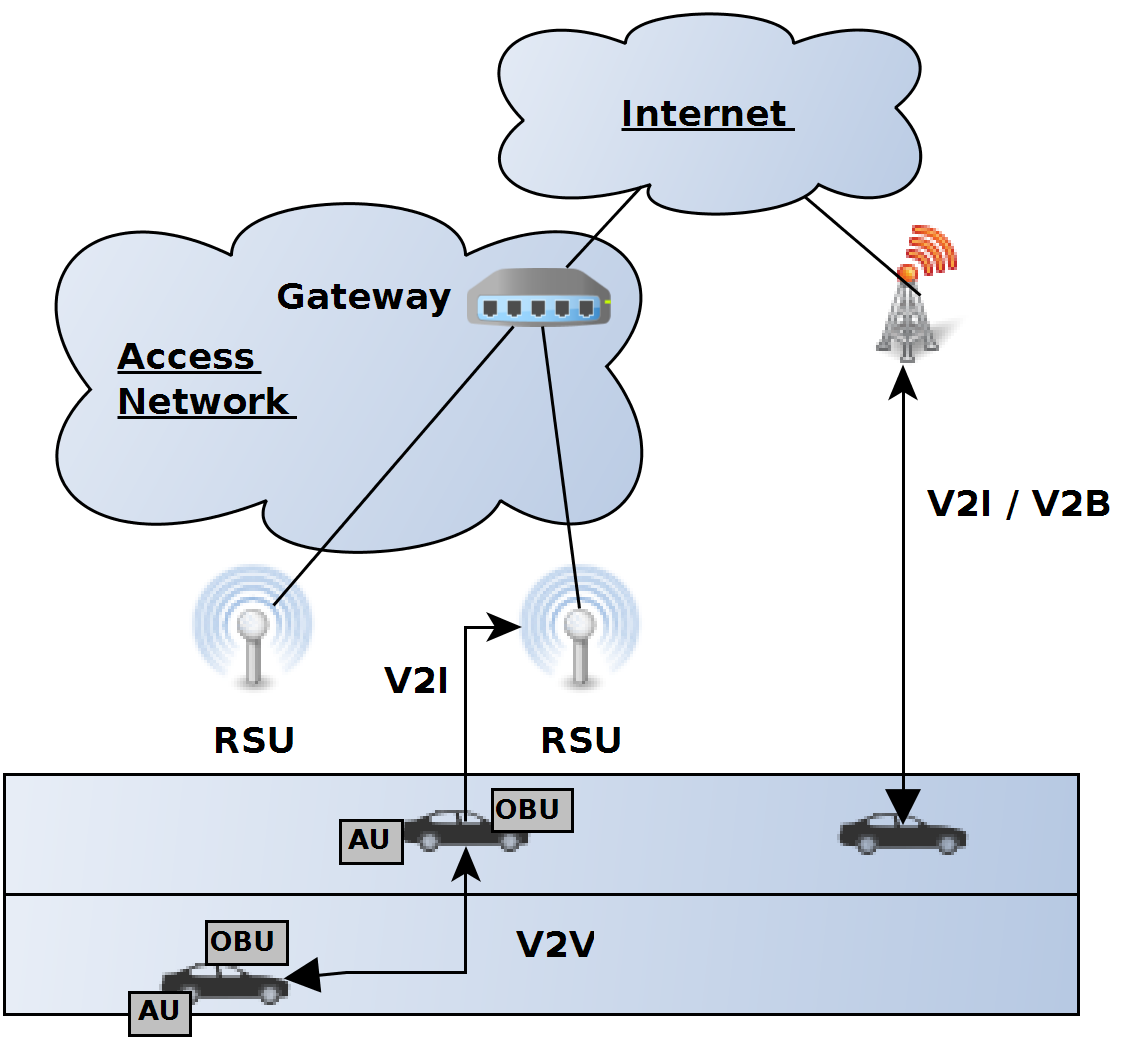
\includegraphics[scale=0.2]{Figures/Vanets.png}
				\caption{General VANET architecture (Based on: \protect\cite{baldessari2007car} and \cite{leiding2016self})}
				\label{fig:vanets}
			\end{figure}			
			Communication in VANETs happens either inside a vehicle between AUs and OBU, wirelessly between different vehicles (V2V) or vehicles and infrastructure (V2I) or between vehicles and the infrastructure via broadband (V2B) \cite{faezipour2012progress}. For authentication purposes, each network participant is equipped with a unique public/private key pair which usually resides in a tamper-proof-device (TPD).
			
		%% ----------------------------------------------------------------
		%% ----------------------------------------------------------------	
		
		\subsection{Related Work}
			\label{ss:related-work}

			\textbf{Work-In-Progress}

			
%			Several other academic as well as non-academic projects experimented with ideas and prototypes of blockchain-based trading platforms that enable the M2M economy. In \cite{leiding2016self}, the authors describe a blockchain solution for a variety of services within vehicular ad-hoc networks (VANETs), e.g., traffic management, toll payment systems, traffic regulation enforcement and more. In 2018, the automotive company got a patent for a very similar idea of traffic marshaling via a blockchain system \cite{macneille2018vehicle}. Chorus technologies \cite{chorusWhitepaper} envisioned a whole library for all types of services and transaction around the ecosystem of autonomous vehicles within VANETs. The authors of \cite{davWhitepaper} propose a solution that allows vehicles to discover, communicate and transact with one another using cryptocurrencies. 
%			\cite{oakenTeslaTollbooth} present a prototype of a blockchain-based toll road system. In 2013, Mike Hearn gave a short talk\footnote{\url{https://www.youtube.com/watch?v=MVyv4t0OKe4}} at the Turing Festival in Edinburgh describing several of these ideas. 
%			
%			Besides the automotive sector, the authors of \cite{sikorski2017blockchain} describe and implement a M2M electricity market for chemical industry where industrial plants are trading electricity with each other via a blockchain platform.
%			
%			The alternative blockchain solution IOTA is offering an IoT market place \cite{iotaMarketplace} for IoT devices where sensor data can be bought and sold using blockchain technology.
%			
%		

%%DAV MVPs \cite{davWhitepaper}
%%MVP#1 World’s first autonomous vehicle to autonomously bid for delivery services, complete them, and get paid using tokens directly to its own wallet.
%%MVP #2 World’s first autonomous vehicle to pay for its own battery replacement using tokens and take off to complete its delivery mission.
%%
%%MVP #3 World’s first autonomous vehicle to pay another autonomous vehicle (robot) using tokens for completing the last mile of a delivery mission.
%%
%%MVP #4 Longest drone delivery flight ever, flying cross-country using the support of multiple DAV battery-changing stations along the way.

% we also have talk about XAIN

		%% ----------------------------------------------------------------
		%% ----------------------------------------------------------------	
	

	%% ----------------------------------------------------------------
	%% ----------------------------------------------------------------

	\section{The Chorus Vision}
		\label{s:section-3}
		
		%%RQ-1: What is the long term vision of Chorus Technology?
		
		Intro

		%foam and localization somewheere here	

		%% ----------------------------------------------------------------
		%% ----------------------------------------------------------------	
		
		\subsection{Use Cases}
			\label{ss:use-cases}

			\textbf{Work-In-Progress}
			
			\subsection{Human to Human}

			\subsection{Human to Vehicle}
		
			\subsection{Vehicle to Vehicle}
			
			\subsection{Vehicle to Infrastructure}					
		
		%% ----------------------------------------------------------------
		%% ----------------------------------------------------------------	


	%% ----------------------------------------------------------------
	%% ----------------------------------------------------------------
	
	
	\section{System Design and Architecture}
		\label{s:section-4}	

		%%RQ-2: What are the critical requirements and the corresponding architecture of the Chorus platform?

		The vision of Chorus outlined in Section \ref{s:section-3} is now analyzed from technical perspective as part of the following section. In order to identify, structure and formalize the critical requirements and stakeholders on an abstract level, we use one part of an Agent-Oriented Modeling (AOM) method \cite{sterling2009art}, i.e., goal models. Section~\ref{ss:requirement-engineering} introduces AOM goal models and the Chorus specific goal model. The produced goal model is used in subsequent Section \ref{ss:component-diagrams} to derive the Chrous system architecture . The resulting system architecture and specifications serve as implementation guidelines. Finally, Section~\ref{ss:smart-contract-lifecycle-management} provides some details on the smart contract lifecycle management within our solution, whereas Section~\ref{ss:library-api} outlines a general outlook on the APIs and how to integrate the Chorus library into external applications.
		
		
		%% ----------------------------------------------------------------
		%% ----------------------------------------------------------------	
		
		\subsection{Functional Goals, Quality Goals, Stakeholders and Requirements}
			\label{ss:requirement-engineering}
						
			In system development and software engieerng, good requirements follow certain characteristics. According to \cite{davis1993software}\cite{ieee1994ieee} requirements address one issue only and are completely specified without missing information. Moreover, they have to be consistent and do not contradict itself, or in correlation with other requirements. Finally, a requirement must also be atomic and without conjunctions \cite{norta2014reference}.
			
			The AOM methodology is a socio-technical requirements-engineering approach used to model complex systems that consist of humans, devices, and software agents. An AOM goal model enables both, technical- and non-technical stakeholders, to capture and understand the functional- and non-functional requirements of a complex system. Figure \ref{fig:aom-notaion-elements} depicts the three main elements that an AOM goal model comprises in order to capture the system requirements and goals. Roles of involved entities are represented in form of sticky men, whereas functional requirements are depicted as parallelograms. Functional requirements are also referred to as goals. Non-functional requirements are depicted as clouds and refer to quality goals of the modeled software system. The AOM goal model follows a tree-like hierarchy with the root value proposition of the modeled system at the top. Subsequently, this main goal is decomposed into sub-goals where each sub-goal represents an aspect for achieving its parent goal \cite{marshall2014agent}. The goals are further decomposed into multi-layered sub-goals until the lowest atomic level is reached. Additionally, roles and quality goal may be assigned to goals and are inherited to lower-level goals.

			\begin{figure}[H]
				\centering
				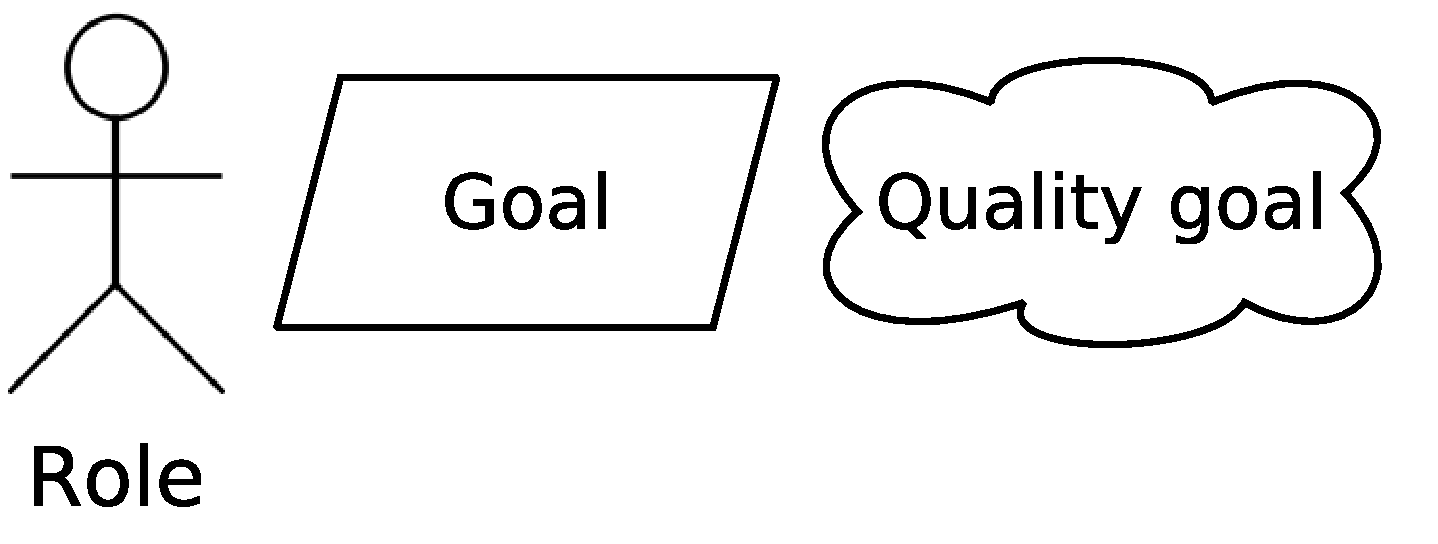
\includegraphics[scale=0.2]{Figures/20180426_AOM-notation.pdf}
				\caption{Selection of AOM notation elements.}	
				\label{fig:aom-notaion-elements}
			\end{figure}	
			
			%% ----------------------------------------------------------------
			%% ----------------------------------------------------------------	
					
			\subsubsection{Top-Level AOM Goal Model}
				\label{sss:top-level-goal-model}

				\begin{figure}[H]
					\centering
					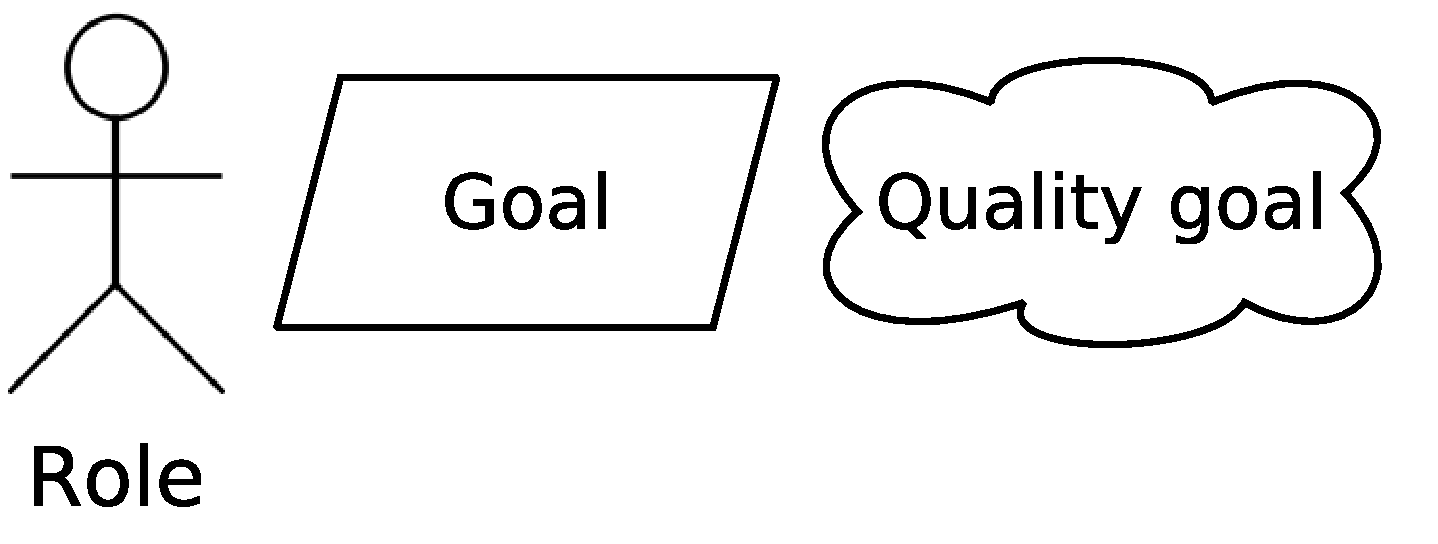
\includegraphics[scale=0.2]{Figures/20180426_AOM-notation.pdf}
					\caption{Caption.}	
					\label{fig:top-level-aom-goal-model}
				\end{figure}

			
			%% ----------------------------------------------------------------
			%% ----------------------------------------------------------------	
					
			\subsubsection{Refined AOM Goal Model}				
				\label{sss:refined-goal-model}			

				\begin{figure}[H]
					\centering
					
\includegraphics[scale=0.4]{Figures/Dummy.jpg}
					\caption{Caption.}	
					\label{fig:refined-aom-goal-model}
				\end{figure}
	
			%% ----------------------------------------------------------------
			%% ----------------------------------------------------------------				

		%% ----------------------------------------------------------------
		%% ----------------------------------------------------------------	
		
		\subsection{Component Diagrams}
			\label{ss:component-diagrams}

			The abstract system- and business architecture is derived from the functional- and non-function requirements of the AOM goal model presented earlier. The services are powered by a service-oriented architecture (SOA) that is comprised of different designated components. Each of these components is self-contained, well-defined components and provides a specific set of services \cite{erl2005service}\cite{perrey2003service}. Dedicated services and components may also consist of other underlying sub-services \cite{rosen2012applied}. 
			
			In the following, a technology-agnostic UML-component-diagram representation is used to illustrate the system architecture \cite{booch1996unified}\cite{specification2007omg}. The UML notation elements used to model the architecture are presented in Figure \ref{fig:uml-component-diagram-overview}. In UML, components are represented as rectangular boxes and labeled either with the keyword \textit{component}, or with the component icon in the right-hand upper corner. A component may consists of further sub-components and is implemented by one, or more classes, or objects. Moreover, components are reusable and communicate via two types of interfaces as illustrated in Figure \ref{fig:uml-component-diagram-overview}. Small squares depict ports that are attached to the border of components and expose required and provided interfaces. Ports may also specify inputs and outputs as they operate uni-, or bi-directionally \cite{booch1996unified}\cite{specification2007omg}. Once more, sticky men are used to depict entities and their interactions with the system. 
			
			\begin{figure}[H]
				\centering
				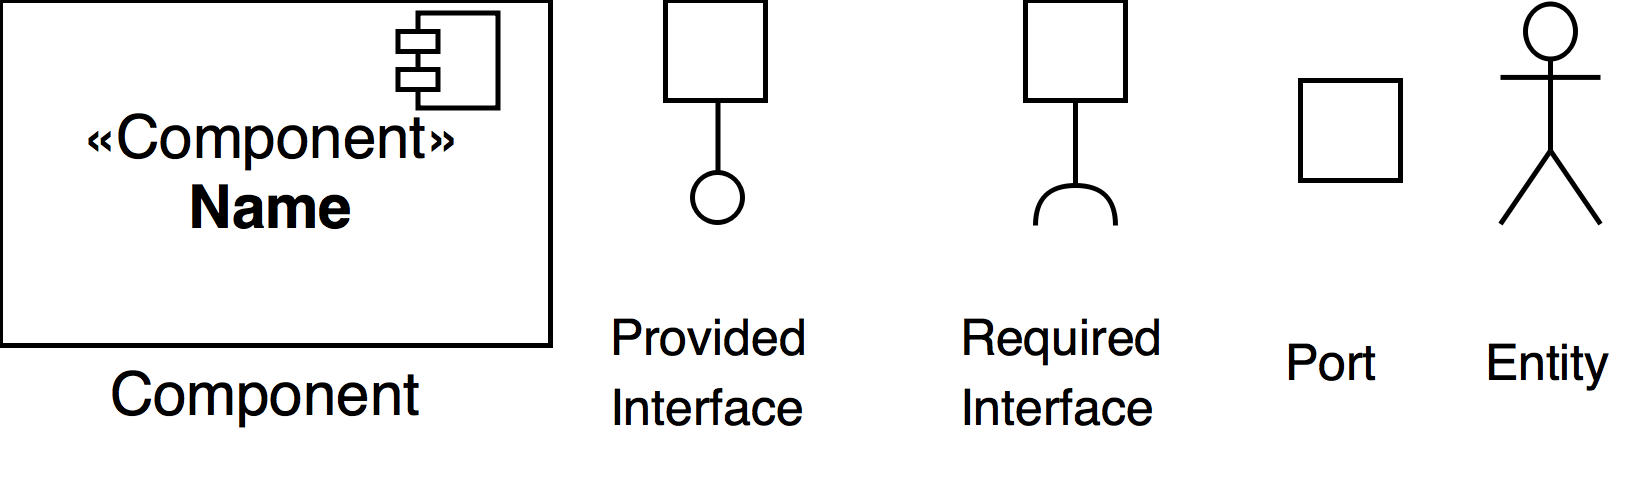
\includegraphics[scale=0.15]{Figures/UML-notation-elements.png}
				\caption{UML-component diagram notation elements.}	
				\label{fig:uml-component-diagram-overview}
			\end{figure}	
			
			The remainder of this section first introduces an abstract high-level overview of the system architecture and components. Afterwards, further illustration present selected sub-components of our architecture.

			%% ----------------------------------------------------------------
			%% ----------------------------------------------------------------	

			\subsubsection{High-Level Architecture}
				\label{sss:high-level-architecture}
			
			%% ----------------------------------------------------------------
			%% ----------------------------------------------------------------	
			

		%	\subsubsection{X}
		%		\label{sss:X}
			
			%% ----------------------------------------------------------------
			%% ----------------------------------------------------------------	
			
			


		%% ----------------------------------------------------------------
		%% ----------------------------------------------------------------	

		\subsection{Smart Contract Lifecycle Management}
			\label{ss:smart-contract-lifecycle-management}

			\textbf{Work-In-Progress}
			
			%			The lifecycle of a micro lending contract is divided into the following stages: a) preparatory, b) negotiation, c) contract execution d) rollback and e) a contract expiry stage. During the preparatory stage, information about the involved entities, such as names and addresses are incorporated into the contract. In addition, the conditions of the requested loans are formally defined by specifying, e.g, the size of the loan, chosen currency, runtime and interest rates. The conditions of the requested loan mainly depend on information available to the lender, such as financial data gathered during previous interactions and transactions, personal data and information from social media. In case the borrower and the lender agree on the negotiated conditions, both parties sign the contract and express their approval - if no agreement is reached, a contract rollback is triggered. After signing the agreement, the contract execution phase is triggered and the lender transfers the loan to the borrower as illustrated in Figure \ref{fig:running-case-illustration}. Afterwards, the lender can use the loan to expand, or start a business. 
			%
			%			The micro lending contract terminates, or expires either after the defined loan timespan, or when the contract is prematurely terminated. The borrower pays back the loan either in separate rates, or as a whole, depending on the defined conditions. In addition, the lender also receives a fee, or an interest rate from the borrower for providing the loan. In case the borrower fulfills all his/her duties, the lender might provide a larger loan in the future based on the positive credit history of the borrower. Everex does not operate on the basis of P2P loans and instead invests its own aggregated capital to provide globally accessible credit services. Nevertheless, it is up to each Cryptocash owner to lend his/her own tokens to other users.	

		%% ----------------------------------------------------------------
		%% ----------------------------------------------------------------	
		
		\subsection{Library / API}
			\label{ss:library-api}				

			\textbf{Work-In-Progress}
			
		%% ----------------------------------------------------------------
		%% ----------------------------------------------------------------	

	%% ----------------------------------------------------------------
	%% ----------------------------------------------------------------
	
	\section{System Engagement Processes}
		\label{s:section-5}	
	
		%% RQ-3: What are the system-engagement processes for the stakeholders?
	
		Intro
		
		%describe processes here similar to evx paper

		%% ----------------------------------------------------------------
		%% ----------------------------------------------------------------	

		\subsection{Sequence Diagrams | or BPMN representation of Processes}

			\textbf{Work-In-Progress}

			\begin{figure}[H]
				\centering
				
\includegraphics[scale=0.4]{Figures/Dummy.jpg}
				\caption{Caption.}	
				\label{fig:sequence-diagram-1}
			\end{figure}


		%% ----------------------------------------------------------------
		%% ----------------------------------------------------------------	
		
		\subsection{Auction Algorithm}
			\label{ss:auchtion-algorithm}				

			\textbf{Work-In-Progress}

			\begin{figure}[H]
				\centering
				
\includegraphics[scale=0.4]{Figures/Dummy.jpg}
				\caption{Caption.}	
				\label{fig:auction-algorithm}
			\end{figure}

		%% ----------------------------------------------------------------
		%% ----------------------------------------------------------------	

		\subsection{Token Economics and Value Proposition}

			\textbf{Work-In-Progress}
					
		%% ----------------------------------------------------------------
		%% ----------------------------------------------------------------	

	%% ----------------------------------------------------------------
	%% ----------------------------------------------------------------

	\section{Prototype and Feasibility Study}
		\label{s:section-6}	
			
		Intro
		
		%% ----------------------------------------------------------------
		%% ----------------------------------------------------------------	
		
		\subsection{Prototype}
			\label{ss:protoype}				

			\textbf{Work-In-Progress}
			
					
		%% ----------------------------------------------------------------
		%% ----------------------------------------------------------------	
		
		\subsection{Evaluation}
			\label{ss:evaluation}				

			\textbf{Work-In-Progress}
			
					
		%% ----------------------------------------------------------------
		%% ----------------------------------------------------------------			

	%% ----------------------------------------------------------------
	%% ----------------------------------------------------------------

	\section{Discussion}
		\label{s:section-7}	
		
		Intro

		%% ----------------------------------------------------------------
		%% ----------------------------------------------------------------	
		
		\subsection{Critical Analysis}
			\label{ss:critical-analysis}
							
			\textbf{Work-In-Progress}		
		
		%% ----------------------------------------------------------------
		%% ----------------------------------------------------------------			
		
		\subsection{Related Work}
			\label{ss:competitor-analysis}
			
			%Competitor analysis (will)				

			\textbf{Work-In-Progress}
		
		%% ----------------------------------------------------------------
		%% ----------------------------------------------------------------					
	
	%% ----------------------------------------------------------------
	%% ----------------------------------------------------------------

	\section{Conclusion and Future Work}
		\label{s:section-8}	

		We conclude ...
		
		\textbf{Work-In-Progress}		
		
		
		%Future Work
		%	- mention the academic M2M paper?
		%	- chorus long term vision
				
	%% ----------------------------------------------------------------
	%% ----------------------------------------------------------------


	\label{Bibliography}
	\bibliographystyle{splncs03}
	\bibliography{Bibliography}
	
	%% ----------------------------------------------------------------
	%% ----------------------------------------------------------------	



	%
\end{document}
